%\documentclass[12pt]{article}
%\usepackage{amsmath}
%\usepackage{geometry}
%\usepackage{graphicx}
%\usepackage{float}
%\geometry{a4paper, portrait, margin=1in}

%	PACKAGES AND OTHER DOCUMENT CONFIGURATIONS
%----------------------------------------------------------------------------------------

\documentclass[12pt]{scrartcl} % Font size

%%%%%%%%%%%%%%%%%%%%%%%%%%%%%%%%%%%%%%%%%
% Wenneker Assignment
% Structure Specification File
% Version 2.0 (12/1/2019)
%
% This template originates from:
% http://www.LaTeXTemplates.com
%
% Authors:
% Vel (vel@LaTeXTemplates.com)
% Frits Wenneker
%
% License:
% CC BY-NC-SA 3.0 (http://creativecommons.org/licenses/by-nc-sa/3.0/)
% 
%%%%%%%%%%%%%%%%%%%%%%%%%%%%%%%%%%%%%%%%%

%----------------------------------------------------------------------------------------
%	PACKAGES AND OTHER DOCUMENT CONFIGURATIONS
%----------------------------------------------------------------------------------------

\usepackage{amsmath, amsfonts, amsthm} % Math packages
\usepackage{physics}%physics packages

\usepackage{listings} % Code listings, with syntax highlighting
%\usepackage{minted}

\usepackage[english]{babel} % English language hyphenation

\usepackage[]{verbatim}
\usepackage{graphicx} % Required for inserting images
\graphicspath{{figures/}{./}} % Specifies where to look for included images (trailing slash required)

\usepackage{booktabs} % Required for better horizontal rules in tables
\usepackage{float}
\usepackage[numbered,framed]{matlab-prettifier}
\lstMakeShortInline"


\numberwithin{equation}{section} % Number equations within sections (i.e. 1.1, 1.2, 2.1, 2.2 instead of 1, 2, 3, 4)
\numberwithin{figure}{section} % Number figures within sections (i.e. 1.1, 1.2, 2.1, 2.2 instead of 1, 2, 3, 4)
\numberwithin{table}{section} % Number tables within sections (i.e. 1.1, 1.2, 2.1, 2.2 instead of 1, 2, 3, 4)

\setlength\parindent{0pt} % Removes all indentation from paragraphs

\usepackage{enumitem} % Required for list customisation
\setlist{noitemsep} % No spacing between list items
\renewcommand{\arraystretch}{1.5}

%----------------------------------------------------------------------------------------
%	DOCUMENT MARGINS
%----------------------------------------------------------------------------------------

\usepackage{geometry} % Required for adjusting page dimensions and margins

\geometry{
	paper=a4paper, % Paper size, change to letterpaper for US letter size
	top=2cm, % Top margin
	bottom=2cm, % Bottom margin
	left=2cm, % Left margin
	right=2cm, % Right margin
	headheight=0.75cm, % Header height
	footskip=1cm, % Space from the bottom margin to the baseline of the footer
	headsep=0.75cm, % Space from the top margin to the baseline of the header
	%showframe, % Uncomment to show how the type block is set on the page
}

%----------------------------------------------------------------------------------------
%	FONTS
%----------------------------------------------------------------------------------------

\usepackage[utf8]{inputenc} % Required for inputting international characters
\usepackage[T1]{fontenc} % Use 8-bit encoding

\usepackage{fourier} % Use the Adobe Utopia font for the document

%----------------------------------------------------------------------------------------
%	SECTION TITLES
%----------------------------------------------------------------------------------------

\usepackage{sectsty} % Allows customising section commands

\sectionfont{\vspace{10pt}\raggedright\normalfont\scshape} % \section{} styling
\subsectionfont{\vspace{10pt}\raggedright\normalfont\bfseries} % \subsection{} styling
\subsubsectionfont{\normalfont\itshape} % \subsubsection{} styling
\paragraphfont{\normalfont\scshape} % \paragraph{} styling

%----------------------------------------------------------------------------------------
%	HEADERS AND FOOTERS
%----------------------------------------------------------------------------------------

\usepackage{scrlayer-scrpage} % Required for customising headers and footers

\ohead*{} % Right header
\ihead*{} % Left header
\chead*{} % Centre header

\ofoot*{} % Right footer
\ifoot*{} % Left footer
%\cfoot*{\pagemark} % Centre footer % Include the file specifying the document structure and custom commands

%----------------------------------------------------------------------------------------
%	TITLE SECTION
%----------------------------------------------------------------------------------------

\title{	
	\normalfont\normalsize
	\text{Memorial University of Newfoundland}
	\vspace{25pt} % Whitespace
	\rule{\linewidth}{0.5pt}\\ % Thin top horizontal rule
	\vspace{20pt} % Whitespace
	{\huge ECE 8600: Design Assignment 1}\\ % The assignment title
	\vspace{12pt} % Whitespace
	\rule{\linewidth}{2pt}\\ % Thick bottom horizontal rule
	\vspace{12pt} % Whitespace
}

\author{\LARGE Aaron Wilcox  } % Your name

\date{\normalsize\today} % Today's date (\today) or a custom date
\lstset{
	style              = Matlab-editor,
	basicstyle         = \mlttfamily,
	escapechar         = ",
	mlshowsectionrules = true,
}

\begin{document}
	
	\maketitle
	\pagebreak
	
		
		
		\section*{Introduction}
		This assignment describes the design of low and highpass filters for the purpose of separating a signal into its high and low dsicrete time frequency components.
		
		\vspace{5mm}
				
		A filter bank using a highpass and a lowpass filter in parallel, was the main idea of the design.

		\section{Scheme 1}
		\subsection{Task a}
		
		The filers to be implemented are:

		\begin{equation*}
				\begin{aligned}
&					H_0 = \frac{1}{2}(1+Z^{-1})\\
&					H_1 = \frac{1}{2}(1-Z^{-1})\\
				\end{aligned}
		\end{equation*}
	
			\vspace{5mm}
		
		MATLAB code for task a is in the section 'a3scheme1ResponsePlots.m' of Appendix A.
		
		\vspace{5mm}
		
		Frequency Response Plots:
		
		\vspace{5mm}
		
		\begin{figure}[H]
			\centering
			\includegraphics[width=12cm]{{figure1.png}}
			\caption{Magnitude of the frequency response for $H_0$}
		\end{figure}
	
		\begin{figure}[H]
			\centering
			\includegraphics[width=12cm]{{figure2.png}}
			\caption{Phase of the frequency response for $H_0$}
		\end{figure}
	
		\begin{figure}[H]
			\centering
			\includegraphics[width=12cm]{{figure3.png}}
			\caption{Magnitude of the frequency response for $H_1$}
		\end{figure}
	
		\begin{figure}[H]
			\centering
			\includegraphics[width=12cm]{{figure4.png}}
			\caption{Phase of the frequency response $H_1$}
		\end{figure}
		
		\subsection*{Task b}
			The filers to be implemented are:
		
		\begin{equation*}
			\begin{aligned}
				&					G_0 = /frac{1}{2}*(1+Z^(-1))\\
				&					G_1 = /frac{1}{2}*(-1+Z^(-1))\\
			\end{aligned}
		\end{equation*}
		
		\vspace{5mm}
		
		MATLAB code for task a (part1Filter.m of Appendix A):
		%\begin{lstlisting}
		\lstinputlisting[language=MATLAB]{a3scheme1GRespPlots.m}
		%\end{lstlisting}
		
		\begin{figure}[H]
			\centering
			\includegraphics[width=12cm]{{figure5.png}}
			\caption{Magnitude of the frequency response for $G_0$}
		\end{figure}
		
		\begin{figure}[H]
			\centering
			\includegraphics[width=12cm]{{figure6.png}}
			\caption{Phase of the frequency response for $G_0$}
		\end{figure}
		
		\begin{figure}[H]
			\centering
			\includegraphics[width=12cm]{{figure7.png}}
			\caption{Magnitude of the frequency response for $G_1$}
		\end{figure}
		
		\begin{figure}[H]
			\centering
			\includegraphics[width=12cm]{{figure8.png}}
			\caption{Phase of the frequency response for $G_1$}
		\end{figure}		
		
		\subsection{Task c: Create a Filter Bank}
		
		The code for the filter bank is listed in branchResponses.m of Appendix A.
	
		
		\begin{figure}[H]
			\centering
			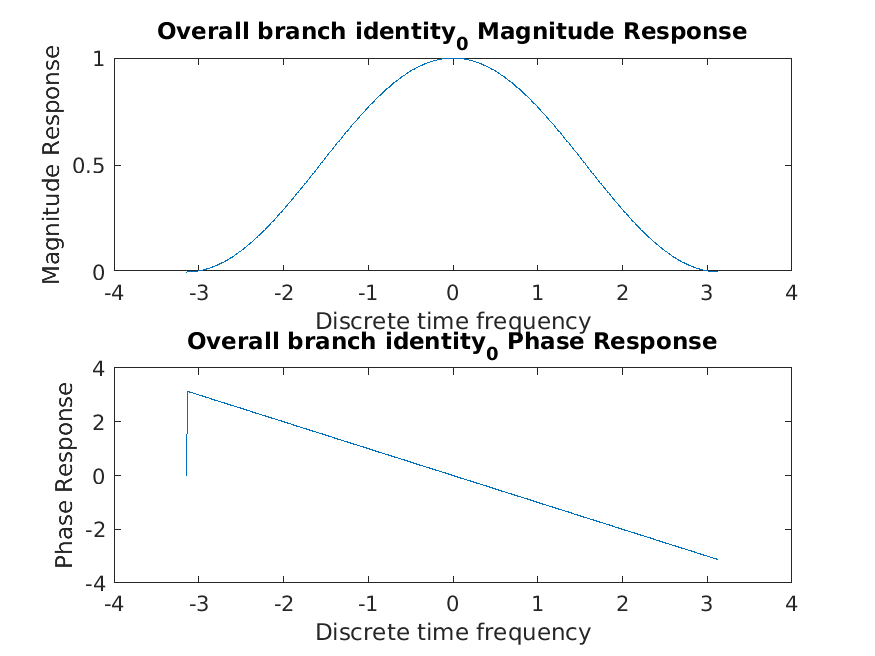
\includegraphics[width=12cm]{figure9.png}
			\caption{The frequency response of the first branch of the parallel filters}
			\end{figure}
		
		\begin{figure}[H]
			\centering
			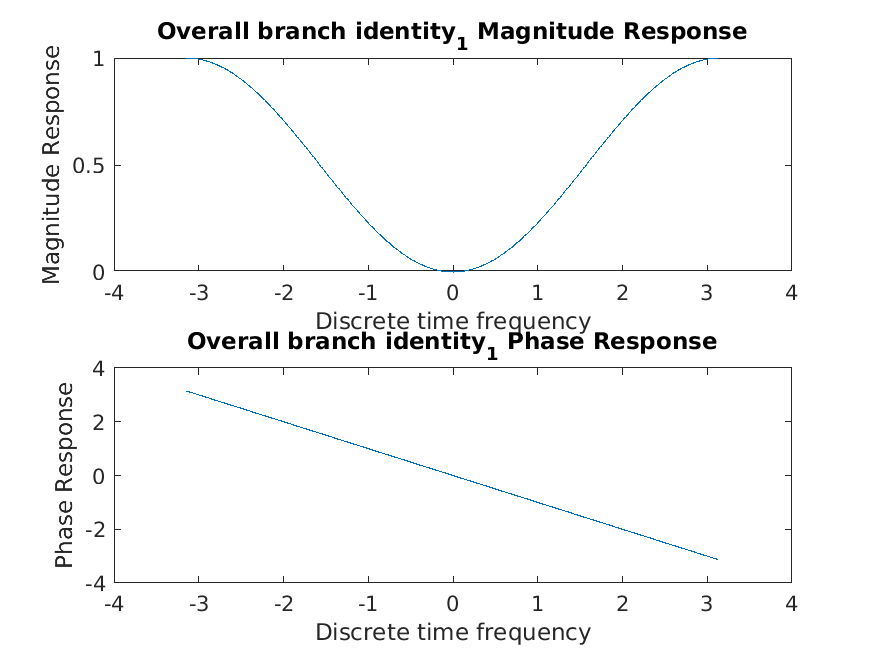
\includegraphics[width=12cm]{figure10.png}
			\caption{The frequency response of the second branch of the parallel filters}
		\end{figure}
	
			\begin{figure}[H]
		\centering
		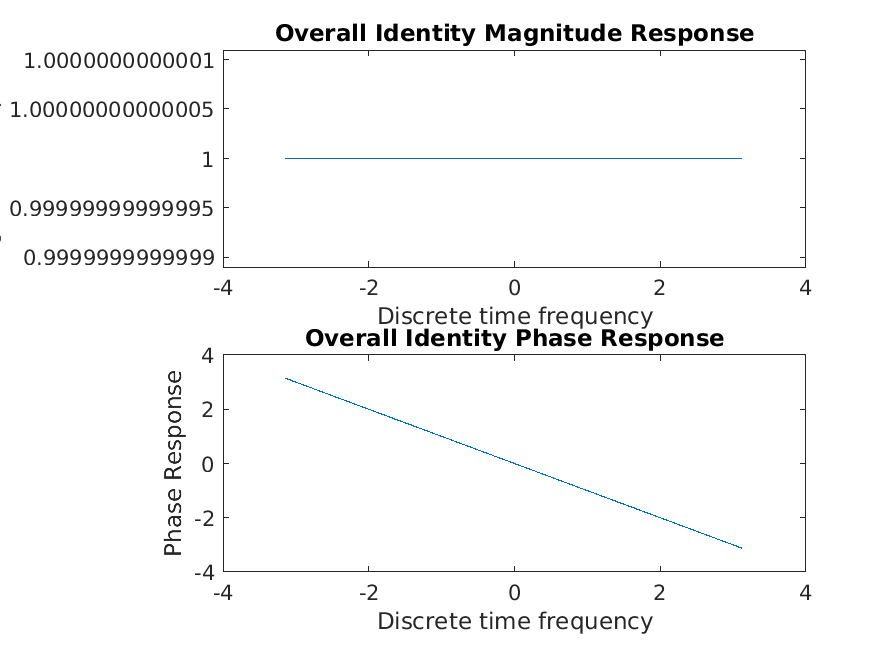
\includegraphics[width=12cm]{figure11.png}
		\caption{The frequency response of the overall filter. Note that the input would be recovered perfectly (with a time delay) with this implementation}
	\end{figure}
	
		
		\subsection{Task d: Test the Filter Bank}
		
			The filter bank was tested by generating 10 sinusoidal inputs, all at different frequencies, and observing the filter output. The details of generating the output can be seen in the code, the main thing to note is that the output was generated using the difference equation of the filter.
		
			\vspace{5mm}
			
			A note about delay aligning:
			
				\vspace{5mm}
				
			There is a MATLAB function called \textbf{finddelay()} that is supposed to find the delay between the input and output signals of a system. I found that inspecting the graphs of the output was a simpler, more accurate way to find the time delay for the case of a single sinusoidal input. The phase of these filters is close to linear, so the input signal and output signal resemble each other quite well (aside from the magnitude change). It should be possible to calculate the time delay because the phase is roughly linear. However, I stuck with my simple method of inspecting the graphs visually. Delays are listed in the below table:
			
						\begin{table}[H]
				\centering
				\begin{tabular}{||c c c ||} 
					\hline
					input signal DT frequency $\omega_0$ & lowpass filter delay & highpass filter delay  \\ [0.5ex] 
					\hline\hline
					$\frac{\pi}{10}$ & 1 & 15 \\
					\hline
					$\frac{3\pi}{10}$ & 6 & 1\\
					\hline
					$\frac{6\pi}{10}$ & 4 & 3\\
					\hline
					$\pi$ & 0 & 0\\ [1ex] 
					\hline
				\end{tabular}
				\caption{output delay for the input signal x = $cos(k \omega_0 n)$ where $\omega_0 = \frac{\pi}{10}$ and $k$ ranges from 1 to 10.}
			\end{table}	
			
			
				\vspace{5mm}
			
			A note about transients:
			
				\vspace{5mm}
			
			My method for determining the length of the transients was the same as my method for finding the time delay between input and output. I inspected the graphs visually and settled on a 
			value of 40 samples to be safe.
			
			\vspace{5mm}
			
			\begin{table}[H]
			\centering
			\begin{tabular}{||c c c ||} 
				\hline
				input signal DT freq & lowpass SNR & highpass SNR  \\ [0.5ex] 
				\hline\hline
				$\frac{\pi}{10}$ & 36.9427 & -38.2942 \\
				\hline
				$\frac{3\pi}{10}$ & 0.0207 & -68.2517\\
				\hline
				$\frac{6\pi}{10}$ & -70.57 & -1.9453\\
				\hline
				$\pi$ & 0 & inf\\ [1ex] 
				\hline
			\end{tabular}
			\caption{test results for the input signal x = $cos(k \omega_0 n)$ where $\omega_0 = \frac{\pi}{10}$ and $k$ ranges from 1 to 10. The -inf result is due to the MSE value for cos(pi) being zero. This is dues to the filter having a passband gain of 1 at DT frequencies of $\pi$}
		\end{table}	
	 
	 	The SNR of 0 that occurs for input frequencies of pi for the lowpass filter, despite perfect attenuation to 0, is due to the MSE being the same as the  square of the ideal value. I chose 0.05*cos(w n) as the ideal value because there would be a 0/0 error otherwise. Instead of 10log(0/0), I end up with 10log(1/1) thus an SNR of 0.
	 	
	 	\vspace{5mm}
	
		All of the time responses were plotted. Note that for the Haar filter the highpass filter passes all frequencies above $\frac{5\pi}{10}$ and the lowpass filter passes all frequencies below to $\frac{5\pi}{10}$, and both filters attenuate the input signal to approximately 1/2 of its input amplitude at an input frequency of $\frac{5\pi}{10}$.

	 	\vspace{5mm}
		
		The Attenuation of the filters is not overly helpful, however. The lowpass filter attenuates signals of frequency $\frac{8\pi}{10}$ and greater by more that 1/2, and the highpass filter attenuates signals of frequency $\frac{2\pi}{10}$ by more than 1/2.
		
			 	\vspace{5mm}
		
		The lowpass and highpass branches' outputs can't simply be taken to be the high and low frequency portions of a given input signal because there would be some content from a signal that is not supposed to be present in the output, present in the output.
	
	
			\begin{figure}[H]
			\centering
			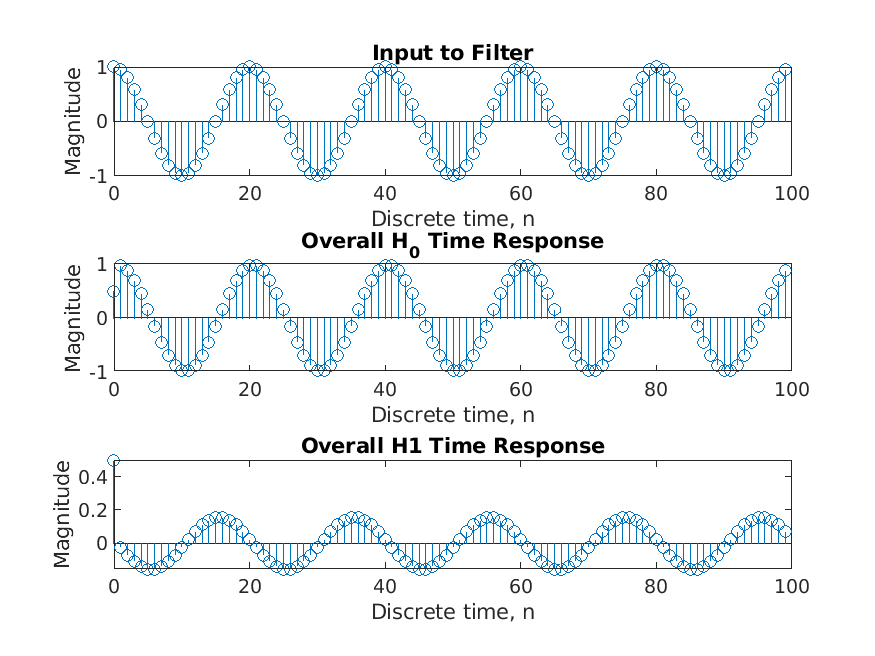
\includegraphics[width=12cm]{figure12.png}
			\caption{The time response of the filters , input frequency is $\pi/10$}
			\end{figure}
	
			\begin{figure}[H]
				\centering
				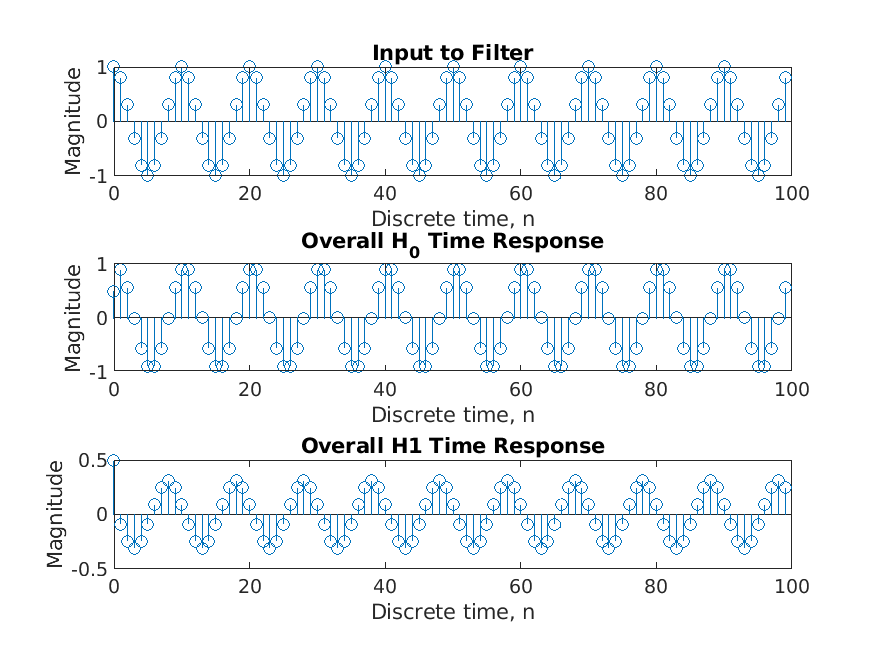
\includegraphics[width=12cm]{figure13.png}
				\caption{The time response of the filters, input frequency is  $2\pi/10$}
			\end{figure}

			\begin{figure}[H]
				\centering
				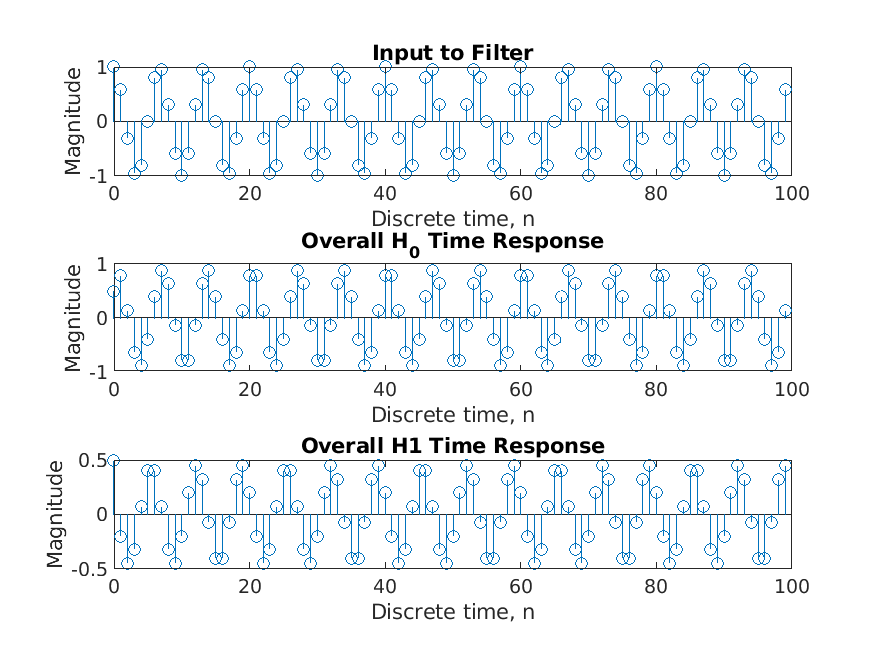
\includegraphics[width=12cm]{figure14.png}
				\caption{The time response of the filters, input frequency is  $3\pi/10$}
			\end{figure}

			\begin{figure}[H]
				\centering
				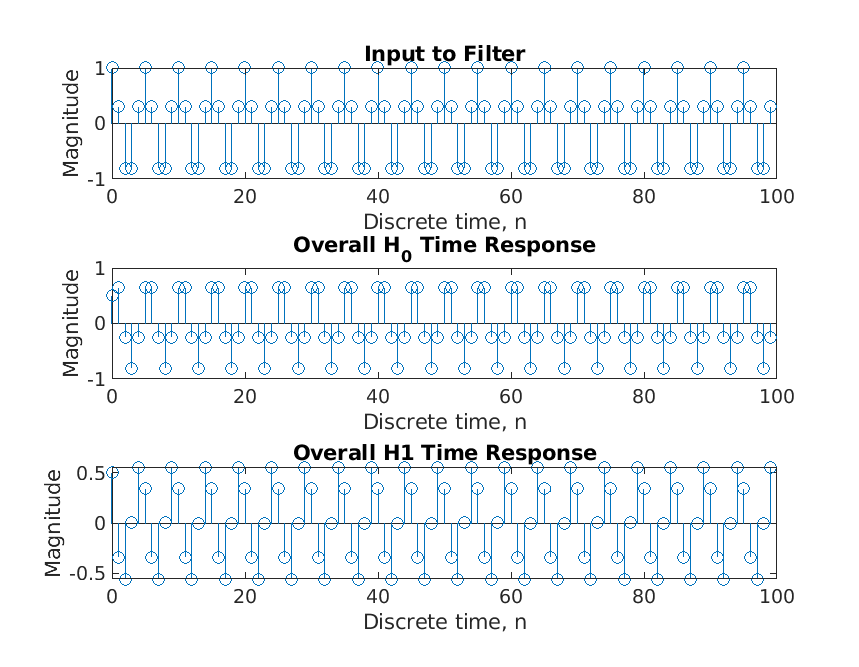
\includegraphics[width=12cm]{figure15.png}
				\caption{The time response of the filters, input frequency is  $4\pi/10$}
			\end{figure}

			\begin{figure}[H]
				\centering
				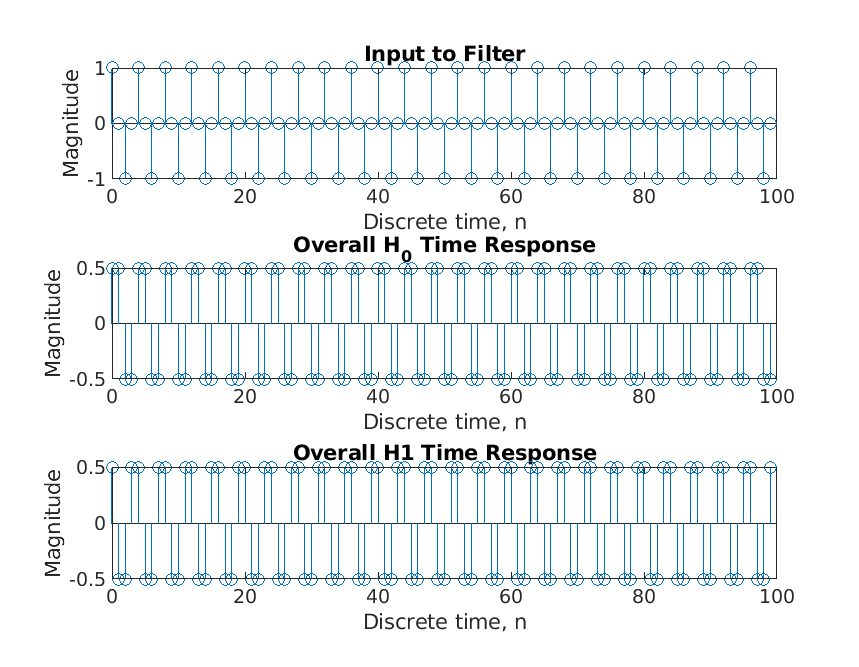
\includegraphics[width=12cm]{figure16.png}
				\caption{The time response of the filters, input frequency is  $5\pi/10$}
			\end{figure}	

			\begin{figure}[H]
				\centering
				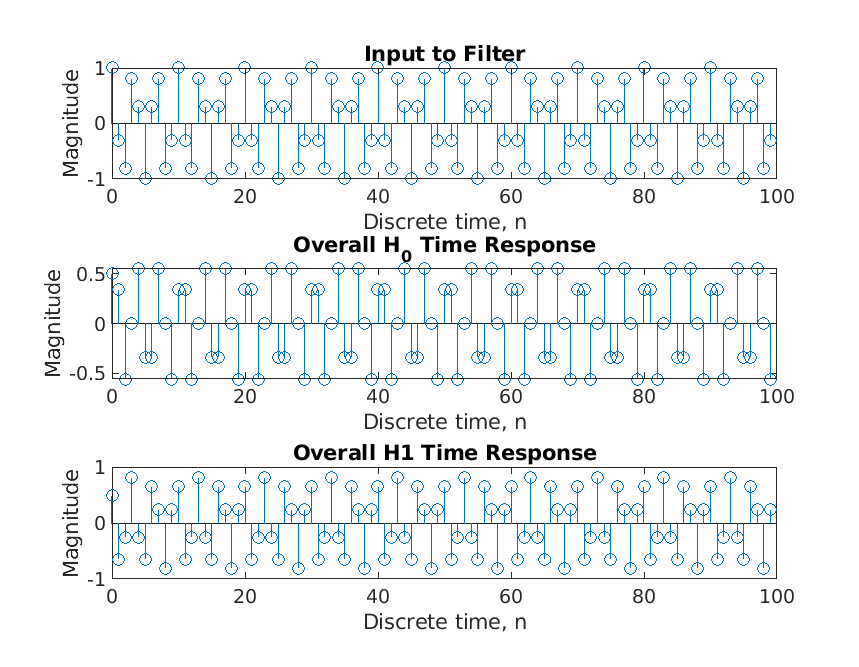
\includegraphics[width=12cm]{figure17.png}
				\caption{The time response of the filters, input frequency is  $6\pi/10$}
			\end{figure}

			\begin{figure}[H]
				\centering
				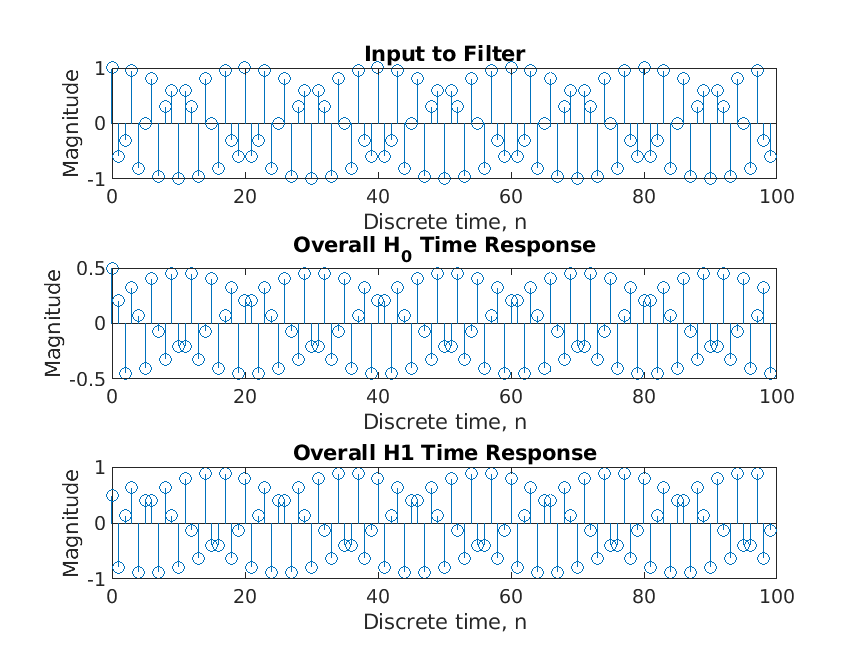
\includegraphics[width=12cm]{figure18.png}
				\caption{The time response of the filters, input frequency is  $7\pi/10$}
			\end{figure}

			\begin{figure}[H]
				\centering
				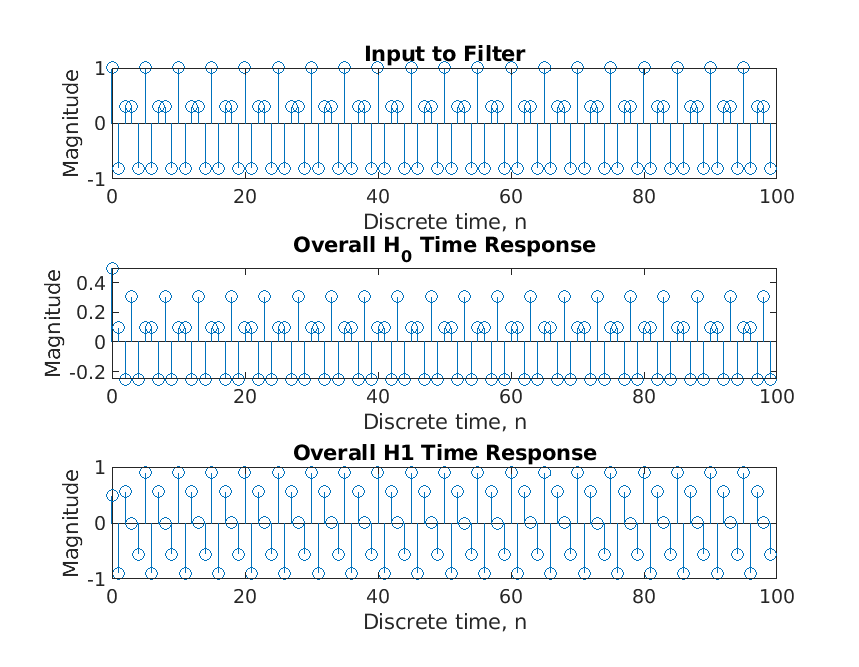
\includegraphics[width=12cm]{figure19.png}
				\caption{The time response of the filters, input frequency is  $8\pi/10$}
			\end{figure}

			\begin{figure}[H]
				\centering
				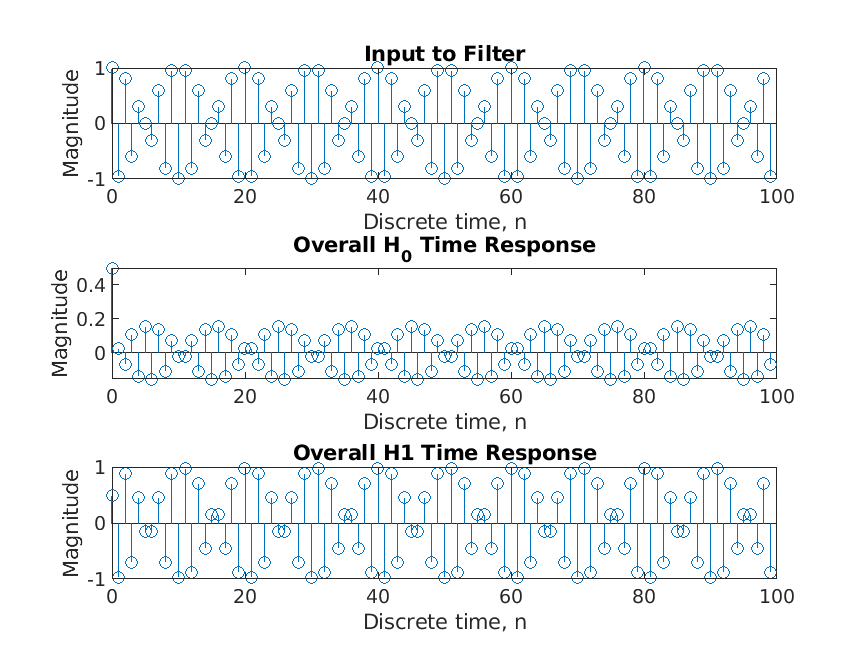
\includegraphics[width=12cm]{figure20.png}
				\caption{The time response of the filters, input frequency is  $9\pi/10$}
			\end{figure}

			\begin{figure}[H]
				\centering
				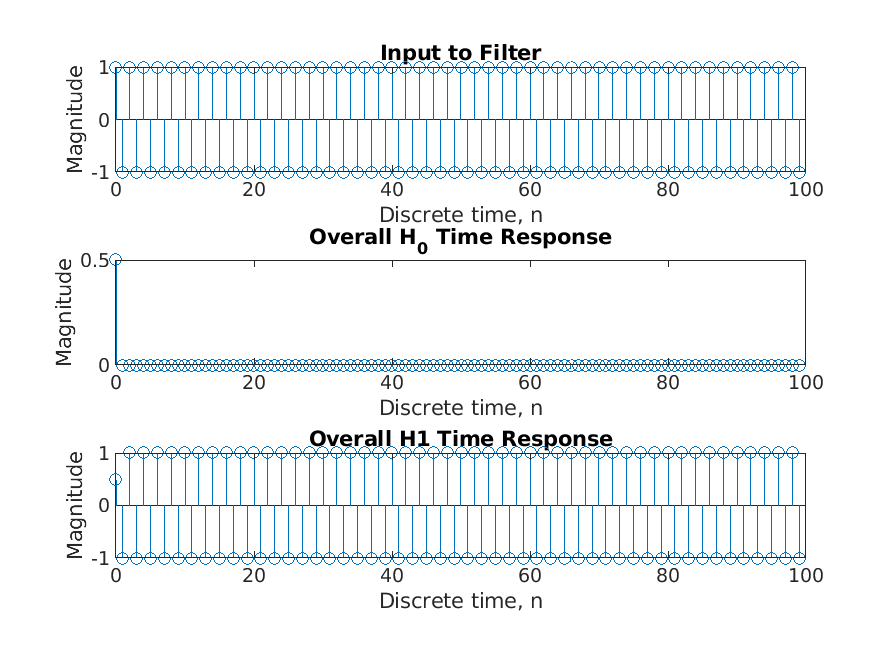
\includegraphics[width=12cm]{figure21.png}
				\caption{The time response of the filters, input frequency is  $10\pi/10$}
			\end{figure}

		
		\section{Scheme 2}
		\subsection{Task a}
		The calculations for the butterworth filter are in Appendix C.
		
				MATLAB code for task A is in  butterworthScheme2.m of Appendix A:

		
		\begin{figure}[H]
			\centering
			\includegraphics[width=12cm]{{figure22.png}}
			\caption{The frequency response for the magnitude squared function, as a sanity check before attempting to generate the butterworth filters}
		\end{figure}
		
		\begin{figure}[H]
			\centering
			\includegraphics[width=12cm]{{figure23.png}}
			\caption{The frequency response for $H_0$, lowpass Butterworth filter}
		\end{figure}
		
		\begin{figure}[H]
			\centering
			\includegraphics[width=12cm]{{figure24.png}}
			\caption{The frequency response for $H_1$, highpass Butterworth filter}
		\end{figure}

		
		\subsection{Task b: Test the Filter Bank}
		
		The filter bank was tested by generating 10 sinusoidal inputs, all at different frequencies, and observing the filter output. The details of generating the output can be seen in the code, the main thing to note is that the output was generated using the difference equation of the filter.
		
		\vspace{5mm}
		
					A note about delay aligning:
		
		\vspace{5mm}
		
		There is a MATLAB function called \textbf{finddelay()} that is supposed to find the delay between the input and output signals of a system. I found that inspecting the graphs of the output
		was a simpler, more accurate way to find the time delay for the case of a single sinusoidal input. The phase of these filters is close to linear, so the input signal and output signal
		resemble each other quite well (aside from the magnitude change). It should be possible to calculate the time delay because the phase is roughly linear. However, I stuck with my simple method of inspecting the graphs visually. Delays are listed in the below table:
		
		\begin{table}[H]
			\centering
			\begin{tabular}{||c c c ||} 
				\hline
				input signal DT frequency $\omega_0$ & lowpass filter delay & highpass filter delay  \\ [0.5ex] 
				\hline\hline
				$\frac{\pi}{10}$ & 5 & 5 \\
				\hline
				$\frac{3\pi}{10}$ & 12 & 0\\
				\hline
				$\frac{6\pi}{10}$ & 2 & 4\\
				\hline
				$\pi$ & 0 & 0\\ [1ex] 
				\hline
			\end{tabular}
			\caption{output delay for the input signal x = $cos(k \omega_0 n)$ where $\omega_0 = \frac{\pi}{10}$ and $k$ ranges from 1 to 10.}
		\end{table}	
		
		
		\vspace{5mm}
		
		A note about transients:
		
		\vspace{5mm}
		
		My method for determining the length of the transients was the same as my method for finding the time delay between input and output. I inspected the graphs visually and settled on a 
		value of 1 sample, which makes sense because this is a FIR filter with a simple difference equation of length 1. 
		
		\vspace{5mm}
		
			\begin{table}[H]
	\centering
	\begin{tabular}{||c c c ||} 
		\hline
		input signal DT freq & lowpass SNR & highpass SNR  \\ [0.5ex] 
		\hline\hline
		$\frac{\pi}{10}$ & 53.0363 & -inf \\
		\hline
		$\frac{3\pi}{10}$ & 67.5711 & -23.0386\\
		\hline
		$\frac{6\pi}{10}$ & -21.9329 & 0.0177\\
		\hline
		$\pi$ & -23.088 & 133.6657\\ [1ex] 
		\hline
	\end{tabular}
	\caption{test results for the input signal x = $cos(k \omega_0 n)$ where $\omega_0 = \frac{\pi}{10}$ and $k$ ranges from 1 to 10. The highpass filter attenuates low frequencies well and passes high frequencies, the lowpass filter attenuates high frequencies well and passes low frequencies}
\end{table}	
	
	All of the time responses were plotted. Note that for the butterworth filter, there are 2
	discrete time frequencies where the transition from signals that classified as low frequency 
	pass over to being classified as high frequency signals. These frequencies are: 

	\vspace{5mm}
	
	- $\frac{4\pi}{10}$
	
	\vspace{5mm}
	
	- $\frac{5\pi}{10}$
		
	\vspace{5mm}
	
	This observation is obvious from figures 2.7 and 2.8. In both cases, the input signal is only attenuated to approximately 1/2 of its input amplitude by one of the 2 filters. In figure 2.7, the $\frac{4\pi}{10}$ signal is not fully attenuated by the lowpass filter, however the highpass filter does attenuate it. In figure 2.8, the $\frac{5\pi}{10}$ signal is not fully attenuated by the highpass filter, however the lowpass filter does attenuate it.
	
		\vspace{5mm}
	
	If this filter were used to segment signals, one way to deal with this would be to classify the signals based on if \textbf{either} of the filters attenuates them significantly.

		\vspace{5mm}
	
	For instance in the case of $\frac{4\pi}{10}$, that frequency would be classified as low frequency because it is attenuated almost entirely by the highpass filter.

	\vspace{5mm}
	
	The opposite case would be true for $\frac{5\pi}{10}$. It would be a high frequency component by the same logic.
	
	\vspace{5mm}
	
	As far as using the output of either branch goes, the following are some relevant notes:
	
	The lowpass and highpass branches' outputs can simply be taken to be the high and low frequency portions of a given input signal because there would only be content from a signal that is lower than $\frac{6\pi}{10}$ present in the lowpass output, and only content from a signal that is higher than $\frac{5\pi}{10}$ present in the highpass output. These observations are clear from the plots 2.4 to 2.13.
	
	
		\begin{figure}[H]
			\centering
			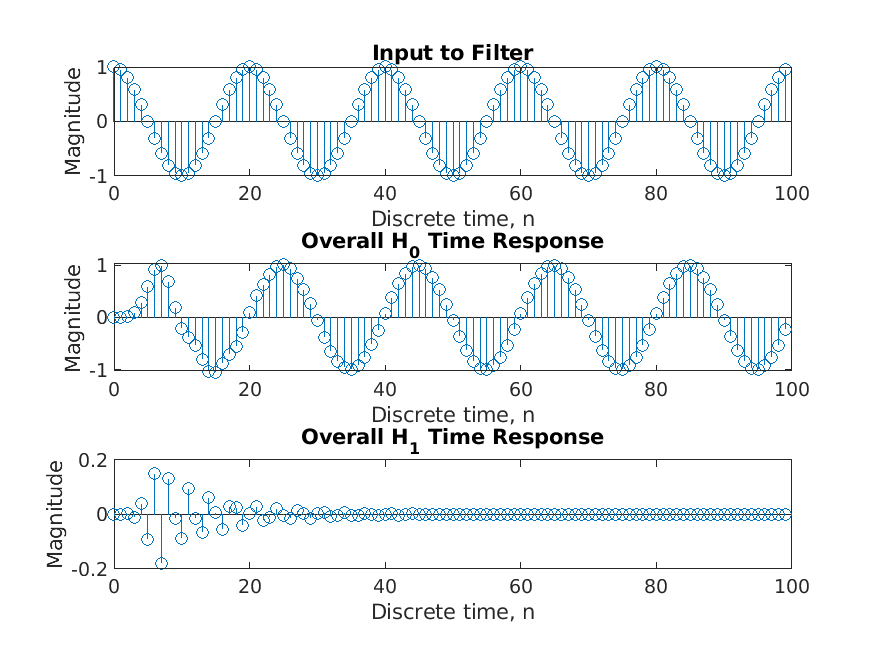
\includegraphics[width=12cm]{figure26.png}
			\caption{The time response of the filters , input frequency is $\pi/10$}
		\end{figure}
		
		\begin{figure}[H]
			\centering
			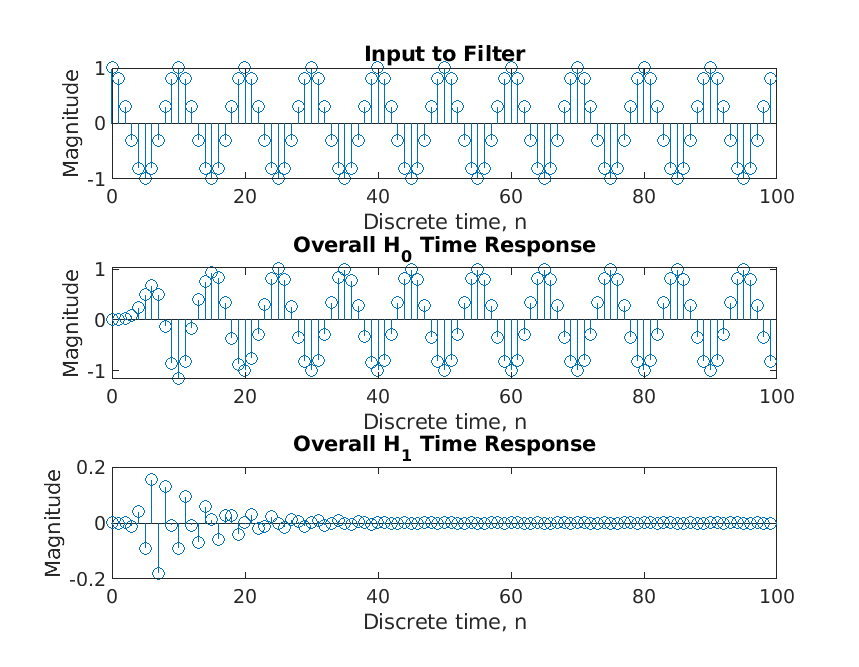
\includegraphics[width=12cm]{figure27.png}
			\caption{The time response of the filters, input frequency is  $2\pi/10$}
		\end{figure}
		
		\begin{figure}[H]
			\centering
			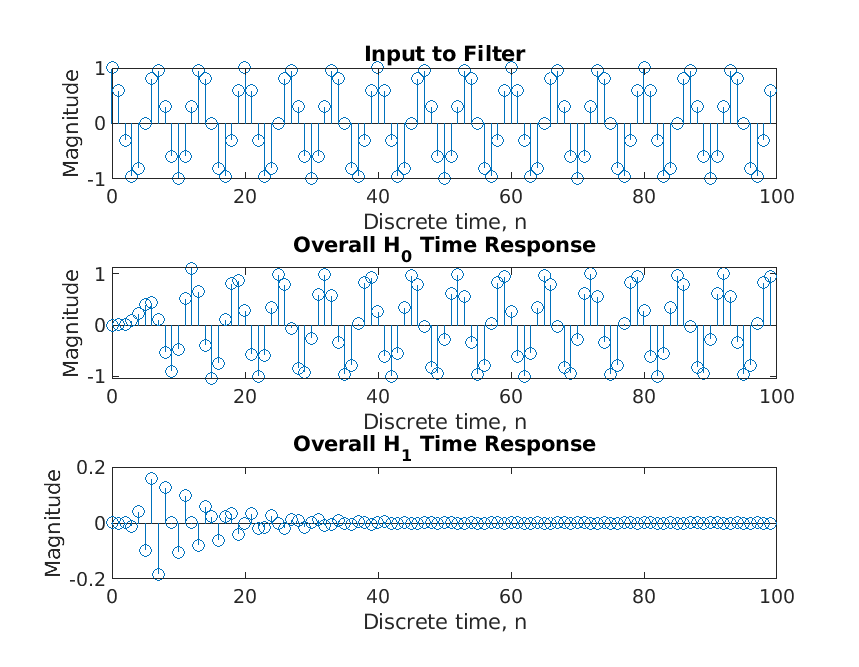
\includegraphics[width=12cm]{figure28.png}
			\caption{The time response of the filters, input frequency is  $3\pi/10$}
		\end{figure}
		
		\begin{figure}[H]
			\centering
			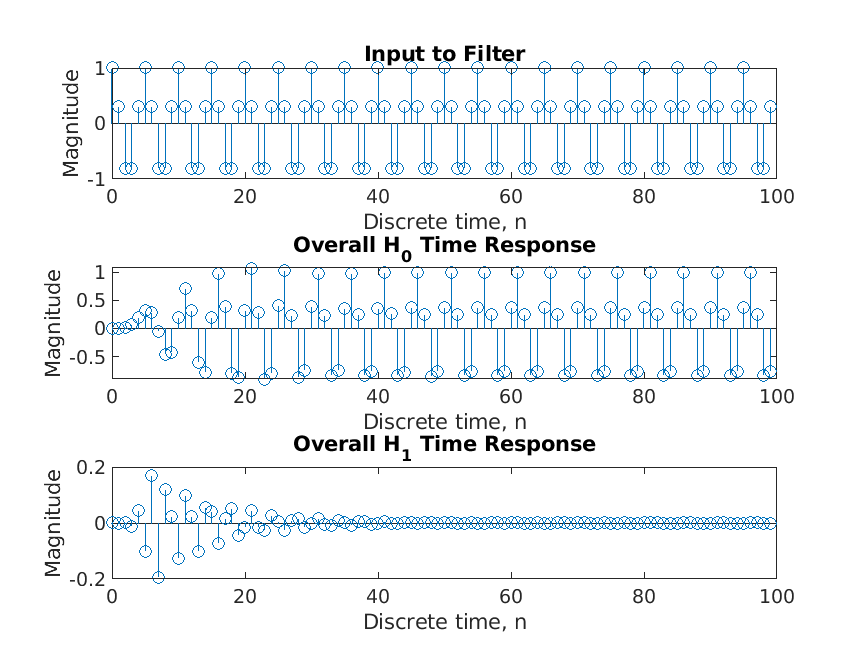
\includegraphics[width=12cm]{figure29.png}
			\caption{The time response of the filters, input frequency is  $4\pi/10$}
		\end{figure}
		
		\begin{figure}[H]
			\centering
			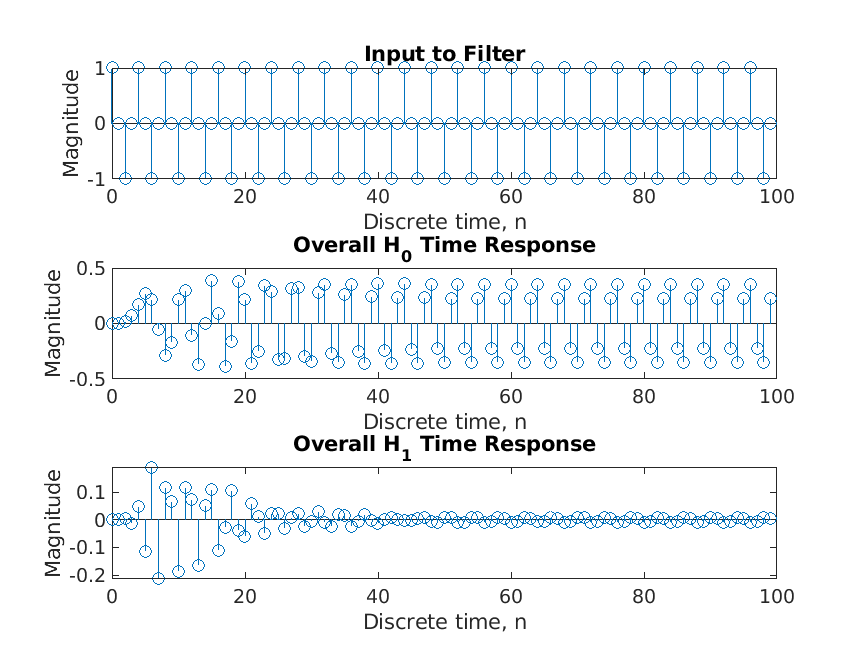
\includegraphics[width=12cm]{figure30.png}
			\caption{The time response of the filters, input frequency is  $5\pi/10$}
		\end{figure}	
		
		\begin{figure}[H]
			\centering
			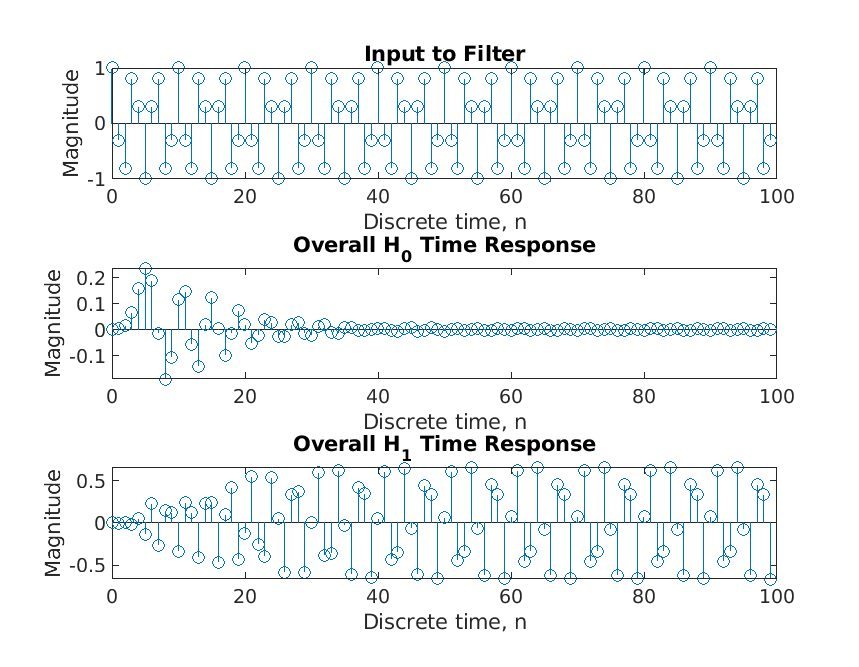
\includegraphics[width=12cm]{figure31.png}
			\caption{The time response of the filters, input frequency is  $6\pi/10$}
		\end{figure}
		
		\begin{figure}[H]
			\centering
			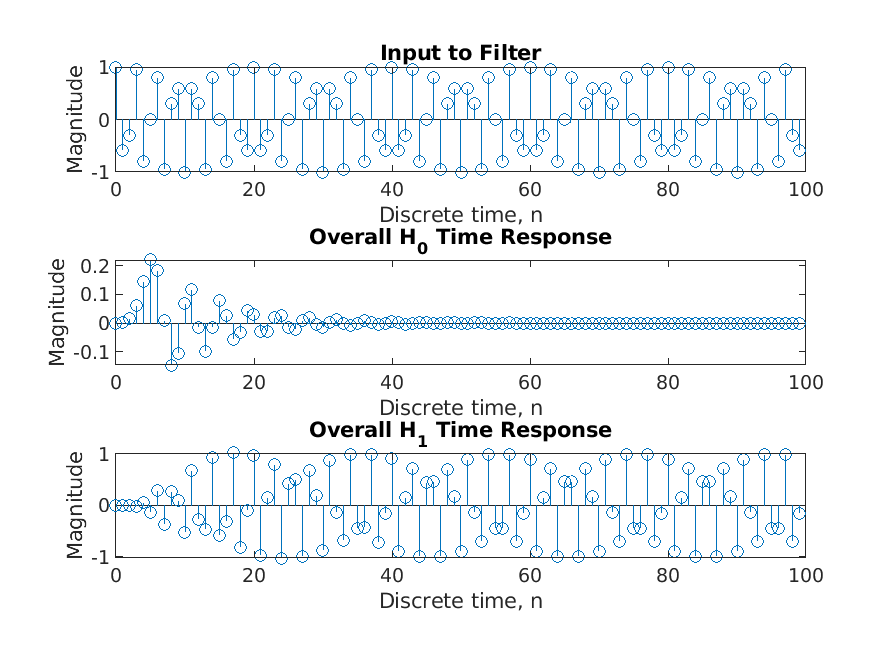
\includegraphics[width=12cm]{figure32.png}
			\caption{The time response of the filters, input frequency is  $7\pi/10$}
		\end{figure}
		
		\begin{figure}[H]
			\centering
			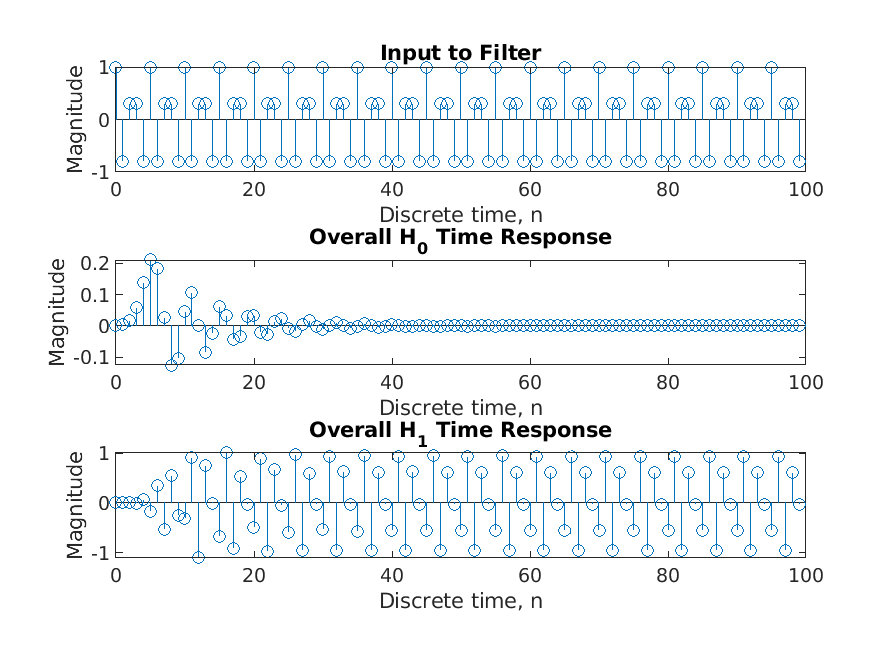
\includegraphics[width=12cm]{figure33.png}
			\caption{The time response of the filters, input frequency is  $8\pi/10$}
		\end{figure}
		
		\begin{figure}[H]
			\centering
			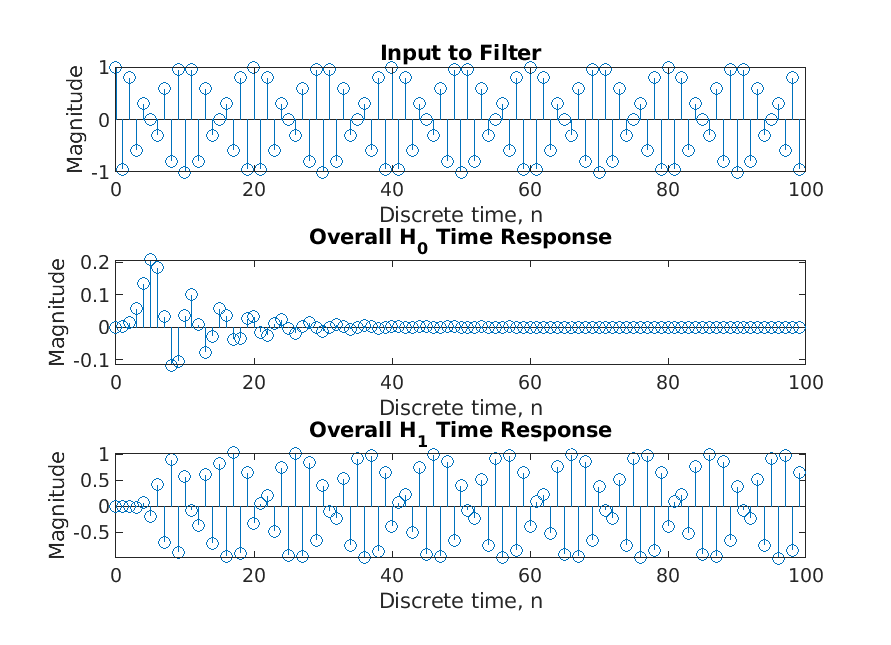
\includegraphics[width=12cm]{figure34.png}
			\caption{The time response of the filters, input frequency is  $9\pi/10$}
		\end{figure}
		
		\begin{figure}[H]
			\centering
			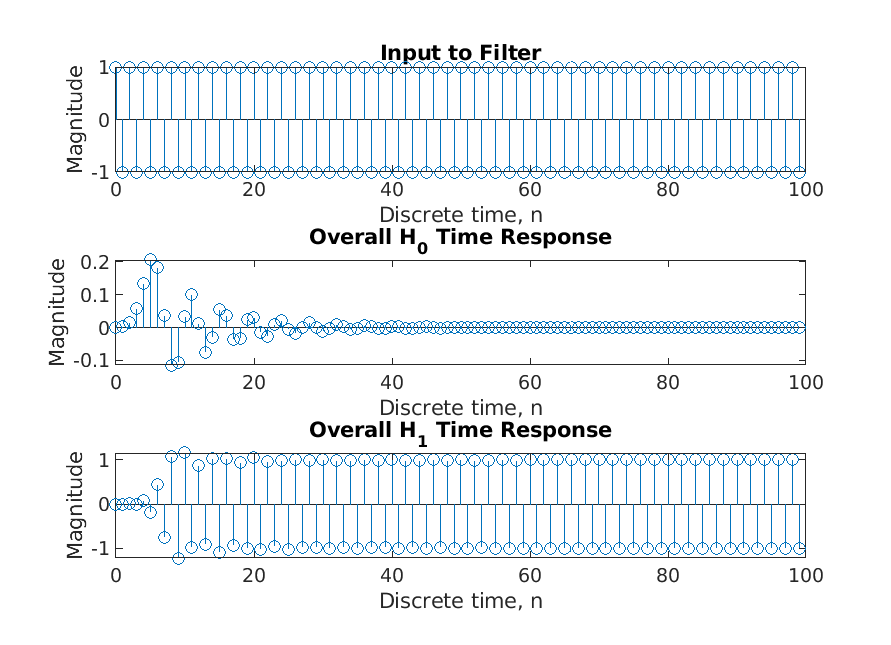
\includegraphics[width=12cm]{figure35.png}
			\caption{The time response of the filters, input frequency is  $10\pi/10$}
		\end{figure}
		
		
		\subsection{Task c: comments on designs}
		
		The butterworth filters of scheme 2 have been shown to be superior to the Haar filters of scheme 1 when it comes to filtering out all of the content of low or high frequencies. This is the objective of the filters, therefore scheme 2 is superior. One nice feature of the Haar filters that is noted in the assignment is that the input can be recovered from the 2 branches, perfectly. This is not the objective however and therefore carries no weight for the desired application.
		
		\section{Appendix A: Main Matlab Scripts}
		
		\subsection{a3scheme1ResponsePlots.m}
							\lstinputlisting[language=MATLAB]{a3Scheme1ResponsePlots.m}
		\subsection{a3scheme1GRespPlots.m}
							\lstinputlisting[language=MATLAB]{a3scheme1GRespPlots.m}
		\subsection{branchResponses.m}							
							\lstinputlisting[language=MATLAB]{branchResponses.m}		
		\subsection{butterworthScheme2.m}							
							\lstinputlisting[language=MATLAB]{butterworthScheme2.m}							
		\subsection{testHaarFilters.m}											
							\lstinputlisting[language=MATLAB]{testHaarFilters.m}
		\subsection{testIIRfilters.m}							
							\lstinputlisting[language=MATLAB]{testIIRfilters.m}
							
		\section{Appendix B: Auxillary Functions Called in main Scripts }
		
				\subsection{plotResp.m}
					\lstinputlisting[language=MATLAB]{plotResp.m}
				\subsection{ccde.m}							
					\lstinputlisting[language=MATLAB]{ccde.m}			
					
		\section{Appendix C: Calculations for Lowpass Butterworth Filter}
		\begin{figure}[h]
			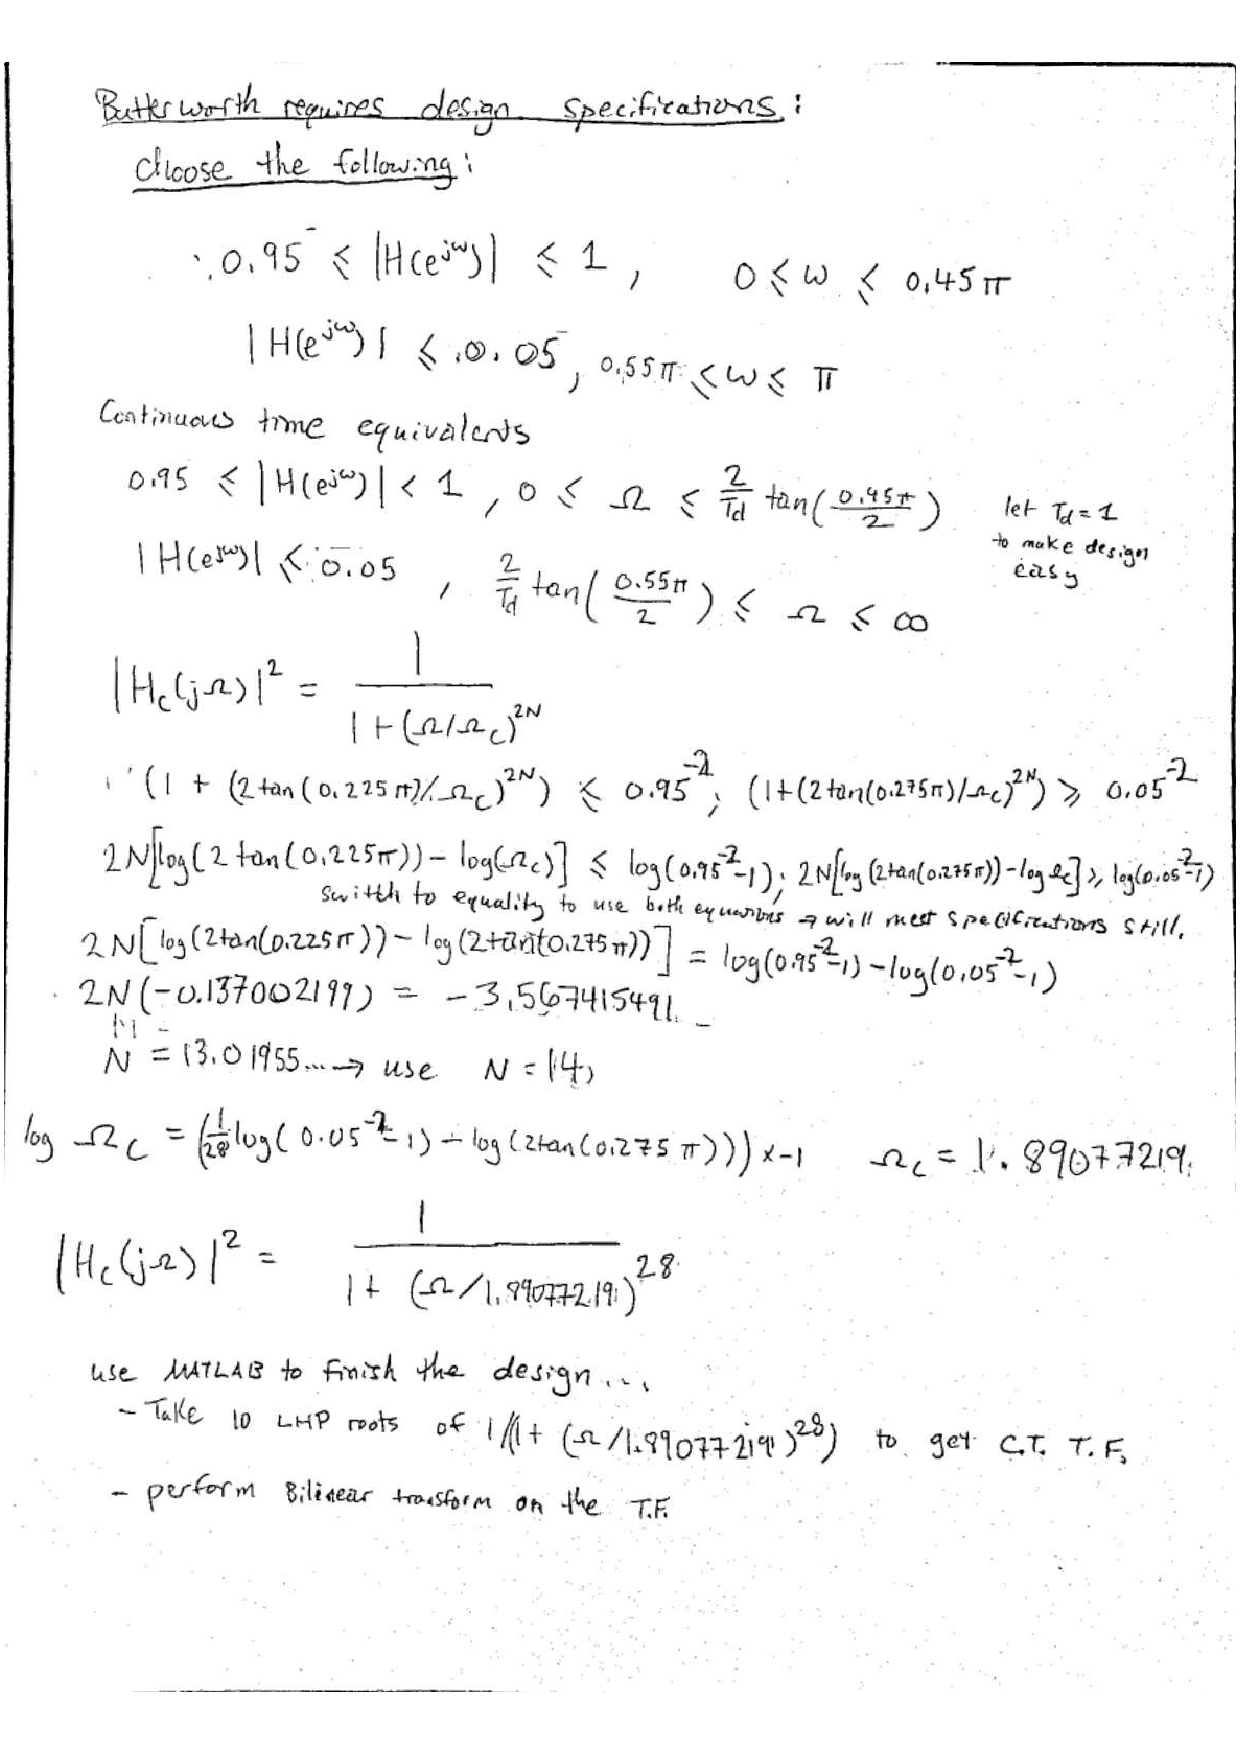
\includegraphics[width=15cm]{butterDesign.pdf}
		\end{figure}
	\end{document}
